\subsubsection{Lavpasfilter}
For at undersøge, hvilken betydning det digitalt filtrede signal har i forhold til det samplede signal, visualiseres disse. De samplede signaler er fra pilotforsøget, som er beskrevet i \autoref{sec:pilotforsoeg}. Signalerne sendes til mikrokontrollen via en UART-forbindelse, hvorved den retunerede værdi modtages og visualiseret i MATLAB, hvilket fremgår af \autoref{fig:lavpas_imp}.

\begin{figure}[H]
\centering
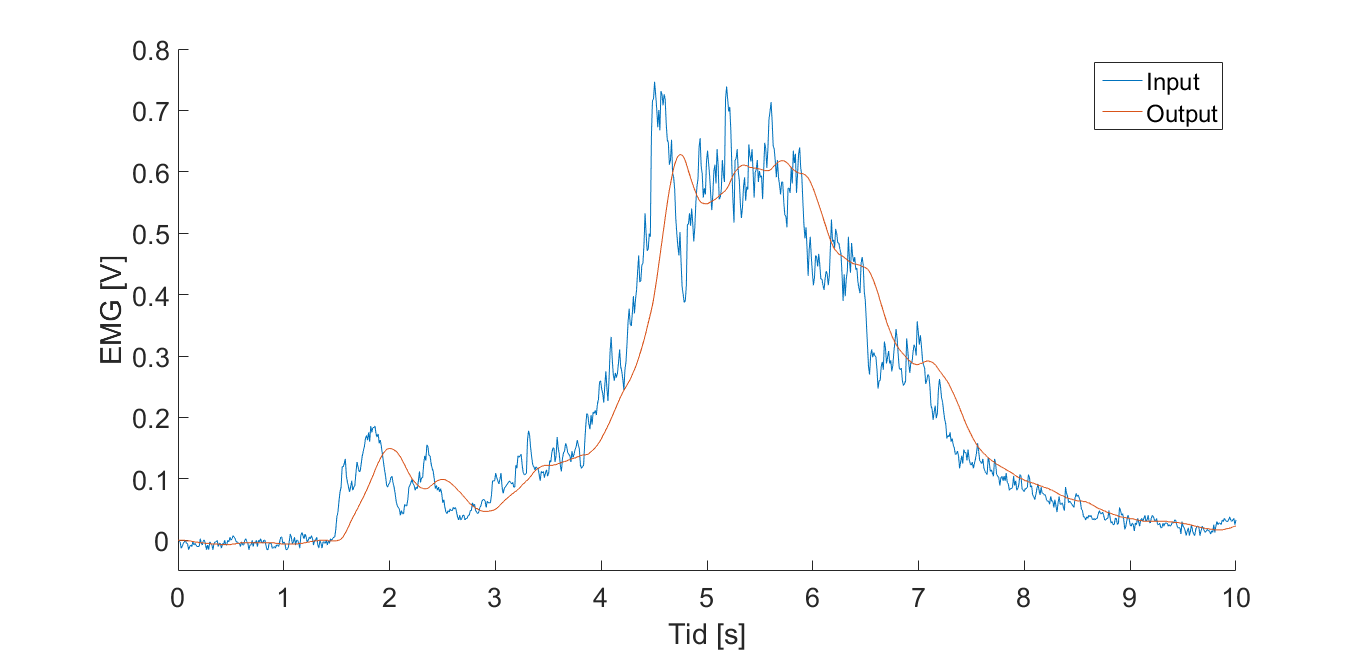
\includegraphics[width=1\textwidth]{figures/EMG_test}
\caption{Den blå graf illustrerer et samplede muskelsignal og den røde graf illustrerer et digitalt filtrede muskelsignal.}
\label{fig:lavpas_imp}
\end{figure}

\noindent
Figuren illustrerer, at inputsignalet følger det samplede signal dog med forsinkelse, for at teste forsinkelsen i det filteret eksekveres, defineres en debug-pin. Denne pin sættes høj før funktionskaldet og lav efter funktionskaldet. For at måle, hvor længe pinen er høj, tilsluttes et oscilloskop. Ud fra dette kan der aflæses en forsinkelse på $175~\mu~s$, hvilket er den forsinkelse der går før data har passeret det digitale filter. Denne forsinkelse vurderes ikke at have nogen signifikant betydning.

For at vurdere om filteret dæmper nok i forhold til de opstillede krav i \autoref{sec:lavpas_krav}, udføres en sweeptest af frekvenser fra $0-15~Hz$ med en funktionsgenerator. Dette frekvensområde er valgt på baggrund af målinger fra \autoref{sec:pilotforsoeg}, hvor det fremgår, at signalet ligger mellem $0,4-10~Hz$.  Da funktionsgeneratoren ikke kan indstilles til en frekvens på $0~Hz$ indstilles denne til $1~\mu~Hz$. Amplituden sættes til 1 $V_{pp}$ med et offset på $1,65~V$, som er det halve af spændingsforsyningen på $3,3~V$. De målte værdier er multipliceret med spændingsforsyningen divideret med ADC'ens arbejdsområde, for således at omregne dette til spænding. Spændingensforsyningen er på $3,3~V$ og ADC'ens arbejdsområde er 2048. Resultatet af sweeptesten fremgår af \autoref{fig:lavps_sweep} \textbf{a)}, mens \textbf{b)} viser kurven for $V_{pp}$ gennem sweppet.

\begin{figure}[H]
\centering
\includegraphics[width=0.8\textwidth]{figures/Lavpass_test}
\caption{Lavpasfiltrering af sweeptest fra 0 til $15~Hz$. Målingen er foretaget med et inputsignal svarende til en sinusbølge med en peak-to-peak på $1~V$. Signalet samples med en frekvens på $100~Hz$. Figur \textbf{a)} viser signalet efter filtrering, mens \textbf{b)} viser $V_{pp}$ gennem en sweeptest. Signalet er opdelt i vinduer af 500 millisekunders varighed og overlapper hinanden med 50 \%.}
\label{fig:lavps_sweep}
\end{figure}

\noindent
En dæmpning på $-3~dB$ for den valgte knækfrekvens på $5~Hz$ bestemmes samt en dekade længere ude svarende til en frekvens på $15~Hz$. Da der anvendes et 2. ordens filter, skal denne frekvens dæmpes ved $-40~dB$. Outputspændingen ved disse dæmpningsfaktorer er udregnet ved \autoref{equ:daempning1} og \autoref{equ:daempning2}. 

\begin{equation} \label{equ:daempning1}
-3~dB = 20 \cdot log_{10} \cdot (\frac{V_{out}}{0,1}) \Rightarrow V_{out} = 0,07 V
\end{equation}
\begin{equation} \label{equ:daempning2}
-40~dB = 20 \cdot log_{10} \cdot (\frac{V_{out}}{0,1}) \Rightarrow V_{out} = 0,01 V
\end{equation}

\noindent
Da målingerne for $V_{pp}$ er downsamplet er det ikke muligt at aflæse nøjagtige værdier, hvorfor der tages udgangspunkt i de nærmeste værdier. Værdierne for $5~Hz$ er $0,06~V$, mens det for $15~Hz$ er $0,008~V$. Afvigelsen fremgår af \autoref{equ:afvigelse1} og \autoref{equ:afvigelse2}.


\begin{equation} \label{equ:afvigelse1}
Afviglese_{5~Hz} = \frac{0,06V-0,07V}{0,07V} = -0,14  = - 14 \%
\end{equation}
\begin{equation} \label{equ:afvigelse2}
Afvigelse_{15~Hz} = \frac{0,008V-0,01V}{0,01V} = -0,20  = -20 \%
\end{equation}

\noindent 
Afvigelserne er for $5~HZ$ 14\%, mens det for $15~Hz$ er 20\%. Dette betyder at filteret ikke dæmper signalet nok. Da målingerne for outputspændingen, målt ved de forskellige frekvenser, ikke er målt nøjagtig aflæst, grundet downsampling, er det forventet, at der er en større afvigelse fra den teoretiske udregning. På baggrund af dette godtages filteret. 

\vspace{3mm}
\textbf{Opsummering af krav:}
\begin{itemize}
\item[\text{\sffamily \checkmark}] Skal følge inputsignalet mest muligt  
\item[\text{\sffamily \checkmark}] Skal udformes som et Butterworth lavpasfilter
\item[\text{\sffamily \checkmark}] Skal have en knækfrekvens på $5~Hz$
\item[\text{\sffamily \checkmark}] Skal have en filterorden på 2
\end{itemize}